%!TeX root=../sensetop.tex
\chapter[Chapter \thechapter]{}
\lettrine[lraise=0.3]{M}{arianne}, who had never much toleration for any thing like impertinence, vulgarity, inferiority of parts, or even difference of taste from herself, was at this time particularly ill-disposed, from the state of her spirits, to be pleased with the Miss Steeles, or to encourage their advances; and to the invariable coldness of her behaviour towards them, which checked every endeavour at intimacy on their side, Elinor principally attributed that preference of herself which soon became evident in the manners of both, but especially of Lucy, who missed no opportunity of engaging her in conversation, or of striving to improve their acquaintance by an easy and frank communication of her sentiments.

Lucy was naturally clever; her remarks were often just and amusing; and as a companion for half an hour Elinor frequently found her agreeable; but her powers had received no aid from education: she was ignorant and illiterate; and her deficiency of all mental improvement, her want of information in the most common particulars, could not be concealed from Miss Dashwood, in spite of her constant endeavour to appear to advantage. Elinor saw, and pitied her for, the neglect of abilities which education might have rendered so respectable; but she saw, with less tenderness of feeling, the thorough want of delicacy, of rectitude, and integrity of mind, which her attentions, her assiduities, her flatteries at the Park betrayed; and she could have no lasting satisfaction in the company of a person who joined insincerity with ignorance; whose want of instruction prevented their meeting in conversation on terms of equality, and whose conduct toward others made every show of attention and deference towards herself perfectly valueless.

<You will think my question an odd one, I dare say,> said Lucy to her one day, as they were walking together from the park to the cottage—<but pray, are you personally acquainted with your sister-in-law's mother, Mrs Ferrars?>

Elinor \textit{did} think the question a very odd one, and her countenance expressed it, as she answered that she had never seen Mrs Ferrars.

<Indeed!> replied Lucy; <I wonder at that, for I thought you must have seen her at Norland sometimes. Then, perhaps, you cannot tell me what sort of a woman she is?>

<No,> returned Elinor, cautious of giving her real opinion of Edward's mother, and not very desirous of satisfying what seemed impertinent curiosity; <I know nothing of her.>

<I am sure you think me very strange, for enquiring about her in such a way,> said Lucy, eyeing Elinor attentively as she spoke; <but perhaps there may be reasons—I wish I might venture; but however I hope you will do me the justice of believing that I do not mean to be impertinent.>

Elinor made her a civil reply, and they walked on for a few minutes in silence. It was broken by Lucy, who renewed the subject again by saying, with some hesitation,

<I cannot bear to have you think me impertinently curious. I am sure I would rather do any thing in the world than be thought so by a person whose good opinion is so well worth having as yours. And I am sure I should not have the smallest fear of trusting \textit{you}; indeed, I should be very glad of your advice how to manage in such an uncomfortable situation as I am; but, however, there is no occasion to trouble \textit{you}. I am sorry you do not happen to know Mrs Ferrars.>

<I am sorry I do \textit{not},> said Elinor, in great astonishment, <if it could be of any use to \textsc{you} to know my opinion of her. But really I never understood that you were at all connected with that family, and therefore I am a little surprised, I confess, at so serious an inquiry into her character.>

<I dare say you are, and I am sure I do not at all wonder at it. But if I dared tell you all, you would not be so much surprised. Mrs Ferrars is certainly nothing to me at present—but the time \textit{may} come—how soon it will come must depend upon herself—when we may be very intimately connected.>

She looked down as she said this, amiably bashful, with only one side glance at her companion to observe its effect on her.

% \begin{figure}[tbph]
% \centering
% 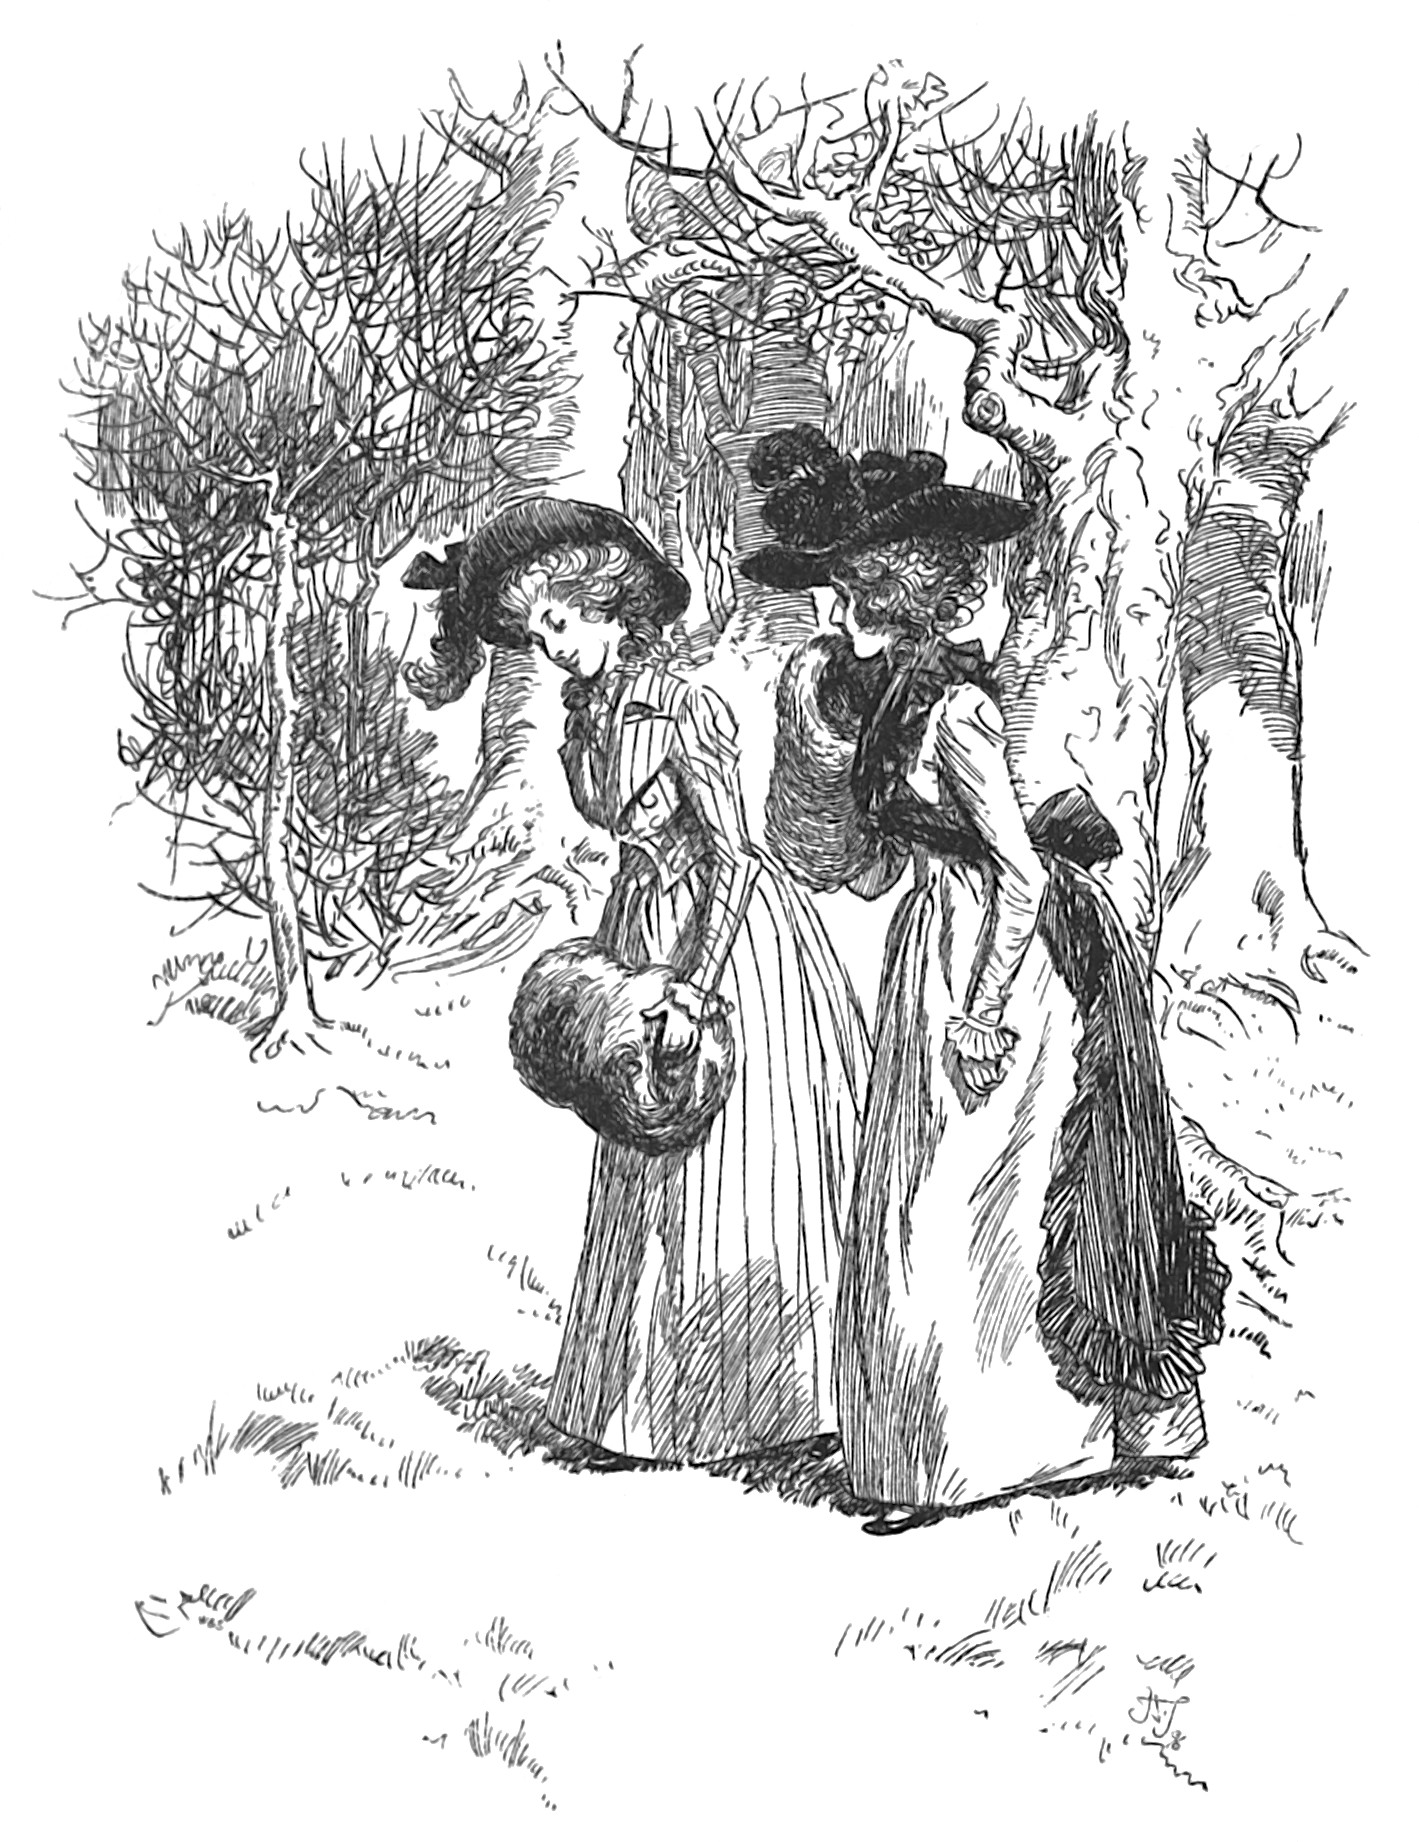
\includegraphics[width=\linewidth]{22amiably}
% \caption{Amiably bashful}
% \end{figure}

\begin{bwbigpic}
	[1.0]
	{22amiably} 
	{Amiably bashful} 
\end{bwbigpic}

<Good heavens!> cried Elinor, <what do you mean? Are you acquainted with Mr Robert Ferrars? Can you be?> And she did not feel much delighted with the idea of such a sister-in-law.

<No,> replied Lucy, <not to Mr \textit{Robert} Ferrars—I never saw him in my life; but,> fixing her eyes upon Elinor, <to his eldest brother.>

What felt Elinor at that moment? Astonishment, that would have been as painful as it was strong, had not an immediate disbelief of the assertion attended it. She turned towards Lucy in silent amazement, unable to divine the reason or object of such a declaration; and though her complexion varied, she stood firm in incredulity, and felt in no danger of an hysterical fit, or a swoon.

<You may well be surprised,> continued Lucy; <for to be sure you could have had no idea of it before; for I dare say he never dropped the smallest hint of it to you or any of your family; because it was always meant to be a great secret, and I am sure has been faithfully kept so by me to this hour. Not a soul of all my relations know of it but Anne, and I never should have mentioned it to you, if I had not felt the greatest dependence in the world upon your secrecy; and I really thought my behaviour in asking so many questions about Mrs Ferrars must seem so odd, that it ought to be explained. And I do not think Mr Ferrars can be displeased, when he knows I have trusted you, because I know he has the highest opinion in the world of all your family, and looks upon yourself and the other Miss Dashwoods quite as his own sisters.>—She paused.

Elinor for a few moments remained silent. Her astonishment at what she heard was at first too great for words; but at length forcing herself to speak, and to speak cautiously, she said, with calmness of manner, which tolerably well concealed her surprise and solicitude—<May I ask if your engagement is of long standing?>

<We have been engaged these four years.>

<Four years!>

<Yes.>

Elinor, though greatly shocked, still felt unable to believe it.

<I did not know,> said she, <that you were even acquainted till the other day.>

<Our acquaintance, however, is of many years date. He was under my uncle's care, you know, a considerable while.>

<Your uncle!>

<Yes; Mr Pratt. Did you never hear him talk of Mr Pratt?>

<I think I have,> replied Elinor, with an exertion of spirits, which increased with her increase of emotion.

<He was four years with my uncle, who lives at Longstaple, near Plymouth. It was there our acquaintance begun, for my sister and me was often staying with my uncle, and it was there our engagement was formed, though not till a year after he had quitted as a pupil; but he was almost always with us afterwards. I was very unwilling to enter into it, as you may imagine, without the knowledge and approbation of his mother; but I was too young, and loved him too well, to be so prudent as I ought to have been. Though you do not know him so well as me, Miss Dashwood, you must have seen enough of him to be sensible he is very capable of making a woman sincerely attached to him.>

<Certainly,> answered Elinor, without knowing what she said; but after a moment's reflection, she added, with revived security of Edward's honour and love, and her companion's falsehood—<Engaged to Mr Edward Ferrars!—I confess myself so totally surprised at what you tell me, that really—I beg your pardon; but surely there must be some mistake of person or name. We cannot mean the same Mr Ferrars.>

<We can mean no other,> cried Lucy, smiling. <Mr Edward Ferrars, the eldest son of Mrs Ferrars, of Park Street, and brother of your sister-in-law, Mrs John Dashwood, is the person I mean; you must allow that I am not likely to be deceived as to the name of the man on who all my happiness depends.>

<It is strange,> replied Elinor, in a most painful perplexity, <that I should never have heard him even mention your name.>

<No; considering our situation, it was not strange. Our first care has been to keep the matter secret. You knew nothing of me, or my family, and, therefore, there could be no \textit{occasion} for ever mentioning my name to you; and, as he was always particularly afraid of his sister's suspecting any thing, \textit{that} was reason enough for his not mentioning it.>

She was silent.—Elinor's security sunk; but her self-command did not sink with it.

<Four years you have been engaged,> said she with a firm voice.

<Yes; and heaven knows how much longer we may have to wait. Poor Edward! It puts him quite out of heart.> Then taking a small miniature from her pocket, she added, <To prevent the possibility of mistake, be so good as to look at this face. It does not do him justice, to be sure, but yet I think you cannot be deceived as to the person it was drew for.—I have had it above these three years.>

She put it into her hands as she spoke; and when Elinor saw the painting, whatever other doubts her fear of a too hasty decision, or her wish of detecting falsehood might suffer to linger in her mind, she could have none of its being Edward's face. She returned it almost instantly, acknowledging the likeness.

<I have never been able,> continued Lucy, <to give him my picture in return, which I am very much vexed at, for he has been always so anxious to get it! But I am determined to set for it the very first opportunity.>

<You are quite in the right,> replied Elinor calmly. They then proceeded a few paces in silence. Lucy spoke first.

<I am sure,> said she, <I have no doubt in the world of your faithfully keeping this secret, because you must know of what importance it is to us, not to have it reach his mother; for she would never approve of it, I dare say. I shall have no fortune, and I fancy she is an exceeding proud woman.>

<I certainly did not seek your confidence,> said Elinor; <but you do me no more than justice in imagining that I may be depended on. Your secret is safe with me; but pardon me if I express some surprise at so unnecessary a communication. You must at least have felt that my being acquainted with it could not add to its safety.>

As she said this, she looked earnestly at Lucy, hoping to discover something in her countenance; perhaps the falsehood of the greatest part of what she had been saying; but Lucy's countenance suffered no change.

<I was afraid you would think I was taking a great liberty with you,> said she, <in telling you all this. I have not known you long to be sure, personally at least, but I have known you and all your family by description a great while; and as soon as I saw you, I felt almost as if you was an old acquaintance. Besides in the present case, I really thought some explanation was due to you after my making such particular inquiries about Edward's mother; and I am so unfortunate, that I have not a creature whose advice I can ask. Anne is the only person that knows of it, and she has no judgment at all; indeed, she does me a great deal more harm than good, for I am in constant fear of her betraying me. She does not know how to hold her tongue, as you must perceive, and I am sure I was in the greatest fright in the world t'other day, when Edward's name was mentioned by Sir John, lest she should out with it all. You can't think how much I go through in my mind from it altogether. I only wonder that I am alive after what I have suffered for Edward's sake these last four years. Every thing in such suspense and uncertainty; and seeing him so seldom—we can hardly meet above twice a-year. I am sure I wonder my heart is not quite broke.>

Here she took out her handkerchief; but Elinor did not feel very compassionate.

<Sometimes.> continued Lucy, after wiping her eyes, <I think whether it would not be better for us both to break off the matter entirely.> As she said this, she looked directly at her companion. <But then at other times I have not resolution enough for it. I cannot bear the thoughts of making him so miserable, as I know the very mention of such a thing would do. And on my own account too—so dear as he is to me—I don't think I could be equal to it. What would you advise me to do in such a case, Miss Dashwood? What would you do yourself?>

<Pardon me,> replied Elinor, startled by the question; <but I can give you no advice under such circumstances. Your own judgment must direct you.>

<To be sure,> continued Lucy, after a few minutes silence on both sides, <his mother must provide for him sometime or other; but poor Edward is so cast down by it! Did you not think him dreadful low-spirited when he was at Barton? He was so miserable when he left us at Longstaple, to go to you, that I was afraid you would think him quite ill.>

<Did he come from your uncle's, then, when he visited us?>

<Oh, yes; he had been staying a fortnight with us. Did you think he came directly from town?>

<No,> replied Elinor, most feelingly sensible of every fresh circumstance in favour of Lucy's veracity; <I remember he told us, that he had been staying a fortnight with some friends near Plymouth.> She remembered too, her own surprise at the time, at his mentioning nothing farther of those friends, at his total silence with respect even to their names.

<Did not you think him sadly out of spirits?> repeated Lucy.

<We did, indeed, particularly so when he first arrived.>

<I begged him to exert himself for fear you should suspect what was the matter; but it made him so melancholy, not being able to stay more than a fortnight with us, and seeing me so much affected. Poor fellow! I am afraid it is just the same with him now; for he writes in wretched spirits. I heard from him just before I left Exeter;> taking a letter from her pocket and carelessly showing the direction to Elinor. <You know his hand, I dare say,—a charming one it is; but that is not written so well as usual. He was tired, I dare say, for he had just filled the sheet to me as full as possible.>

Elinor saw that it \textit{was} his hand, and she could doubt no longer. This picture, she had allowed herself to believe, might have been accidentally obtained; it might not have been Edward's gift; but a correspondence between them by letter, could subsist only under a positive engagement, could be authorised by nothing else; for a few moments, she was almost overcome—her heart sunk within her, and she could hardly stand; but exertion was indispensably necessary; and she struggled so resolutely against the oppression of her feelings, that her success was speedy, and for the time complete.

<Writing to each other,> said Lucy, returning the letter into her pocket, <is the only comfort we have in such long separations. Yes, \textit{I} have one other comfort in his picture, but poor Edward has not even \textit{that}. If he had but my picture, he says he should be easy. I gave him a lock of my hair set in a ring when he was at Longstaple last, and that was some comfort to him, he said, but not equal to a picture. Perhaps you might notice the ring when you saw him?>

<I did,> said Elinor, with a composure of voice, under which was concealed an emotion and distress beyond any thing she had ever felt before. She was mortified, shocked, confounded.

Fortunately for her, they had now reached the cottage, and the conversation could be continued no farther. After sitting with them a few minutes, the Miss Steeles returned to the Park, and Elinor was then at liberty to think and be wretched.